\begin{problem}[h]
<<echo=FALSE>>=
x_outside_square = sample(c(2, 4, 6, 8, 10, 12, 14, 16, 20), 1)#We get a sample among these even numbers
x_inside_square = 3
x_right_tower = x_outside_square*3
result = x_right_tower
fake_result1 = x_outside_square
fake_result2 = x_inside_square
fake_result3 = x_outside_square/2
@
{\bf Trigonometry.} 
If the distance between the towers is $\Sexpr{(x_outside_square)}\sqrt{\Sexpr{(x_inside_square)}}$ m, the hight of the right tower would be?
\begin{center}
    \begin{minipage}{8cm}
        \begin{center}
            \begin{answers}{2}
            \bChoices[random]
                \Ans0 \Sexpr{(fake_result1)}m\eAns
                \Ans0 \Sexpr{(fake_result2)}m\eAns
                %\Ans0 \Sexpr{(fake_result3)}m\eAns
		\Ans0 $\sqrt{\Sexpr{(x_inside_square)}}$m\eAns
                \Ans0 $\Sexpr{(x_outside_square)}\sqrt{\Sexpr{(x_inside_square)}}$m\eAns
                \Ans1 \label{resp3.1} \Sexpr{(result)}m\eAns
                \eFreeze
                \Ans0 None of them\eAns
                \eChoices
            \end{answers} 
        \end{center}
    \end{minipage}
    \begin{minipage}{5cm}
        \begin{center}
            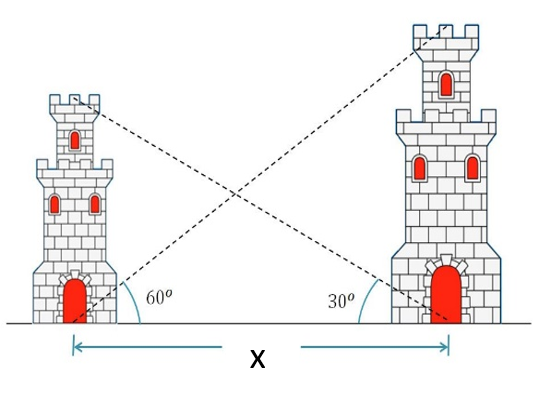
\includegraphics[width=3cm, height=3cm]{two_towers_question.png}
        \end{center}
    \end{minipage}
\end{center}
\begin{solution}
Using the triangle of the right side and the definition of the tangent,\\
$y_{tower}=\tan{60}^{\circ}\cdot\Sexpr{(x_outside_square)}\sqrt{\Sexpr{(x_inside_square)}}m=\Sexpr{(result)}m$\\
Therefore, the right answer is the letter \textbf{(\REF*{resp3.1})}
\end{solution}
\end{problem}
